\documentclass[11pt]{article}

% Change "review" to "final" to generate the final (sometimes called camera-ready) version.
% Change to "preprint" to generate a non-anonymous version with page numbers.
\usepackage[utf8]{inputenc}
\usepackage[]{acl}
\usepackage{times}
\usepackage{latexsym}
\usepackage{dirtree}
\usepackage{listings}
\usepackage{multirow}
\usepackage{graphicx}
\usepackage{natbib}
\usepackage{array}
\usepackage{tikz}
\usepackage{subcaption}
\usepackage{pgfplots}
\usepackage{multicol}
\pgfplotsset{compat=1.17}
\bibliographystyle{plainnat}
\graphicspath{ {./Images/} }

% For proper rendering and hyphenation of words containing Latin characters (including in bib files)

% DISABLE IF WE CAN NOT USE ANOTHER FONT
% I JUST HATE THE DEFAULT FONT - Elite
\usepackage[sfdefault,lf]{carlito}
\renewcommand{\familydefault}{\sfdefault}
\usepackage[T1]{fontenc}
% For Vietnamese characters
% \usepackage[T5]{fontenc}
% See https://www.latex-project.org/help/documentation/encguide.pdf for other character sets

% This assumes your files are encoded as UTF8
\usepackage[utf8]{inputenc}
\usepackage{microtype}
\usepackage{inconsolata}
\usepackage{graphicx}
\definecolor{dkgreen}{rgb}{0,0.6,0}
\definecolor{gray}{rgb}{0.5,0.5,0.5}
\definecolor{mauve}{rgb}{0.58,0,0.82}

\lstset{frame=tb,
  language=python,
  aboveskip=3mm,
  belowskip=3mm,
  showstringspaces=false,
  columns=flexible,
  basicstyle={\small\ttfamily},
  numbers=none,
  numberstyle=\tiny\color{gray},
  keywordstyle={\small\ttfamily},
  commentstyle=\color{dkgreen},
  stringstyle=\color{mauve},
  breaklines=true,
  breakatwhitespace=true,
  tabsize=3
}

% If the title and author information does not fit in the area allocated, uncomment the following
%
%\setlength\titlebox{<dim>}
%
% and set <dim> to something 5cm or larger.


\title{Group 76 Final Report: Classification of Retinal Diseases Using Optical Coherence Tomography (OCT) Images}


\author{Elite Lu, Ishpreet Nagi, Kenneth Ong \\
  \texttt{\{lue13,nagii,salimk4\}@mcmaster.ca} }

%\author{
%  \textbf{First Author\textsuperscript{1}},
%  \textbf{Second Author\textsuperscript{1,2}},
%  \textbf{Third T. Author\textsuperscript{1}},
%  \textbf{Fourth Author\textsuperscript{1}},
%\\
%  \textbf{Fifth Author\textsuperscript{1,2}},
%  \textbf{Sixth Author\textsuperscript{1}},
%  \textbf{Seventh Author\textsuperscript{1}},
%  \textbf{Eighth Author \textsuperscript{1,2,3,4}},
%\\
%  \textbf{Ninth Author\textsuperscript{1}},
%  \textbf{Tenth Author\textsuperscript{1}},
%  \textbf{Eleventh E. Author\textsuperscript{1,2,3,4,5}},
%  \textbf{Twelfth Author\textsuperscript{1}},
%\\
%  \textbf{Thirteenth Author\textsuperscript{3}},
%  \textbf{Fourteenth F. Author\textsuperscript{2,4}},
%  \textbf{Fifteenth Author\textsuperscript{1}},
%  \textbf{Sixteenth Author\textsuperscript{1}},
%\\
%  \textbf{Seventeenth S. Author\textsuperscript{4,5}},
%  \textbf{Eighteenth Author\textsuperscript{3,4}},
%  \textbf{Nineteenth N. Author\textsuperscript{2,5}},
%  \textbf{Twentieth Author\textsuperscript{1}}
%\\
%\\
%  \textsuperscript{1}Affiliation 1,
%  \textsuperscript{2}Affiliation 2,
%  \textsuperscript{3}Affiliation 3,
%  \textsuperscript{4}Affiliation 4,
%  \textsuperscript{5}Affiliation 5
%\\
%  \small{
%    \textbf{Correspondence:} \href{mailto:email@domain}{email@domain}
%  }
%}
\setlength{\parindent}{0pt}
\begin{document}
\maketitle
% \begin{abstract}
% \end{abstract}




% DO NOT REMOVE THIS LINE or else a lot of errors WILL APPEAR for line spacing
\hbadness=100000


\section{Introduction}

Healthcare providers deal with many vision related illnesses such as Diabetic Macular Edema (DME), Choroidal Neovascularization (CNV), and drusen. The utilization of these retinal scans detect and determine these conditions. An issue that arises is the uniqueness of each ailment, as each condition varies in subtle ways. Correctly identifying retinal diseases can prove to be a challenge in a plethora of cases and with approximately 30 million OCT scans performed each year, this process can be time-consuming and labor-intensive for healthcare professionals. By having a classification model that can help speed up this process, healthcare professionals should be able to focus their attention on helping more individuals requiring their aid.

\section{Related Work}

With the rising popularity of Machine Learning (ML) and Deep Learning (DL) in recent years, it is not surprising that many researchers around the world have worked on the classification of retinal diseases using ML and/or DL methods. Most related works have approached the problem by incorporating transfer learning to perform multi-class or binary classification~\citep{Kermany2018-dc, Miladinovic2024-og,Reddy_2025-nr}.

As seen in the notebook created by the Kaggle user Badduri Nagendra Reddy~\citeyearpar{Reddy_2025-nr}, the fine-tuned model based on ResNet50 was able to achieve an impressive 98.97\% final test accuracy on the same dataset as the one used in this project. Similarly, the models defined in the papers typically build upon a pre-trained model, where the authors only unfreeze the weights of the last few layers and add a final classification layer~\citep{Kermany2018-dc,Miladinovic2024-og}.

Additionally, these studies experimented with different base models such as VGG16, InceptionV3, and other variations of ResNet, all of which were able to achieve mid-to-high 90\% accuracy~\citep{9002415,Kermany2018-dc,Miladinovic2024-og}. In contrast, the paper by Özdaş et al.~\citeyearpar{diagnostics13030433} outlined an interesting approach using the Firefly algorithm combined with transfer learning models to extract features from images, followed by classical ML classifiers for binary classification, achieving 95.7\% accuracy on their dataset.

\section{Dataset}

\subsection{Folder Structure}

When downloading the data, the dataset was partitioned as follows:

\dirtree{%
    .1 Dataset.
    .2 test.
    .3 CNV.
    .3 DME.
    .3 DRUSEN.
    .3 NORMAL.
    .2 train.
    .3 CNV.
    .4 augmented.
    .3 DME.
    .4 augmented.
    .3 DRUSEN.
    .4 augmented.
    .3 NORMAL.
    .4 augmented.
    .2 val.
    .3 CNV.
    .3 DME.
    .3 DRUSEN.
    .3 NORMAL.
}

\vspace*{0.1cm}

The new added folders for the training data, augmented, contains the augmented image data for each category. The reason for this will be elaborated in the \textbf{Data Augmentation} section.

\vfill

\subsection{Initial Image Counts}

\begin{center}
    \begin{tabular}{|c|c|c|}
        \hline
        \textbf{Type}          & \textbf{Disease} & \textbf{\# of Images} \\
        \hline
        \multirow{4}{*}{train} & CNV              & 37205                 \\ \cline{2-3}
                               & DME              & 11348                 \\ \cline{2-3}
                               & DRUSEN           & 8616                  \\ \cline{2-3}
                               & NORMAL           & 26315                 \\
        \hline
        \multirow{4}{*}{test}  & CNV              & 242                   \\ \cline{2-3}
                               & DME              & 242                   \\ \cline{2-3}
                               & DRUSEN           & 242                   \\ \cline{2-3}
                               & NORMAL           & 242                   \\
        \hline
        \multirow{4}{*}{val}   & CNV              & 8                     \\ \cline{2-3}
                               & DME              & 8                     \\ \cline{2-3}
                               & DRUSEN           & 8                     \\ \cline{2-3}
                               & NORMAL           & 8                     \\
        \hline
    \end{tabular}
\end{center}

\subsection{Data Augmentation}

One of the encountered problems with the dataset is the class imbalance. As seen in the \textbf{Initial Image Counts} table, the number of images vary drastically. For example, CNV has nearly 4.5 times the amount of images the DRUSEN class has. Because of this, the model will be biased towards the classes with more images, thus resulting in poor performance. To mitigate this, data augmentation was performed on the training dataset to increase the number of images such that each class has the same number of images. This was done by performing the following random actions:

\begin{lstlisting}
augmentation_transforms = transforms.Compose([
        transforms.RandomHorizontalFlip(),
        transforms.RandomRotation(50),
        transforms.RandomResizedCrop(size=224, scale=(0.8, 1.0)),
        transforms.ColorJitter(brightness=0.2, contrast=0.2),
    ])
\end{lstlisting}

This augmentation process includes randomly flipping the image horizontally, randomly rotating the image by up to 50 degrees, randomly cropping and resizing the image, and randomly changing the contrast and brightness of the image. By performing this, not only will the dataset be more robust as a whole, but the model will less likely to overfit or have bias towards a certain class.

As a result, the new image counts after augmentation are as follows:

\vfill

\begin{center}
    \begin{tabular}{|c|c|c|}
        \hline
        \textbf{Type}          & \textbf{Disease} & \textbf{\# of Images} \\
        \hline
        \multirow{4}{*}{train} & CNV              & 37205                 \\ \cline{2-3}
                               & DME              & 37205                 \\ \cline{2-3}
                               & DRUSEN           & 37205                 \\ \cline{2-3}
                               & NORMAL           & 37205                 \\
        \hline
        \multirow{4}{*}{test}  & CNV              & 242                   \\ \cline{2-3}
                               & DME              & 242                   \\ \cline{2-3}
                               & DRUSEN           & 242                   \\ \cline{2-3}
                               & NORMAL           & 242                   \\
        \hline
        \multirow{4}{*}{val}   & CNV              & 8                     \\ \cline{2-3}
                               & DME              & 8                     \\ \cline{2-3}
                               & DRUSEN           & 8                     \\ \cline{2-3}
                               & NORMAL           & 8                     \\
        \hline
    \end{tabular}
\end{center}

This results in the training dataset having a total of 148820 images.

\subsection{Preprocessing}

Each image was loaded from the various folders as a PIL (Pillow, not the Python Imaging Library) Image and then converted to a tensor object. The pipeline varies slightly for the \textit{train} dataset when compared to both \textit{test} and \textit{val} datasets. Both pipelines resized the images to 224 pixels by 224 pixels and normalized them with means [0.485, 0.456, 0.406] and standard deviation (std) of [0.229, 0.224, 0.225]. Since we are using ResNet50 as the base model, the values for the mean and standard deviation come from ImageNet's preset values, which is the dataset that ResNet is being trained on. The only difference in the preprocessing pipeline is that before normalization, the \textit{train} dataset images might be horizontally flipped whereas the image data for the \textit{test} and \textit{val} pipelines is not. This allowed for the training set to have a more robust dataset. However, this is technically not considered an augmentation since no new data was created (no data distribution changes).

\subsection{Annotation}
Each image was labeled with an integer to represent its corresponding disease. The images were already named as DISEASE-\#\#\#\#\#-\#.jpeg and located in their corresponding folders, which allowed for ease of labeling. When assigning labels to the dataset, we use the following mapping:

\begin{center}
    \begin{tabular}{| c | c |}
        \hline \hline
        \textbf{CNV}    & 0 \\
        \hline
        \textbf{DME}    & 1 \\
        \hline
        \textbf{DRUSEN} & 2 \\
        \hline
        \textbf{NORMAL} & 3 \\
        \hline \hline
    \end{tabular}
\end{center}

\section{Features}

\subsection{Data Input}
Since this is a computer vision/image classification task, the features were derived from the pixels of the images. Each pixel was denoted by three values: Red(R), Green(G), and Blue(B). As mentioned previously, each image was cropped and normalized with values corresponding the means and standard deviations for images from ImageNet.

\subsection{Features}
The selection of features was not done directly. This was because it was not required as there are no features to select. Since the pixels are the "feature", this would not be justified. As a result, feature engineering and feature selection was not needed. The same can be said for learning embeddings, as this is not a natural language processing task.

For the output features, there are four main features, which are the four categories of diseases: CNV, DME, DRUSEN, and NORMAL.

\section{Implementation}

\subsection{Learning Model}
Instead of training a model from scratch, a pretrained neural network was used and adapted it to the use case. The pretrained neural network selected was ResNet-50, which was trained on the ImageNet dataset. ResNet-50 is a neural network that is 50 layers deep originally developed by Microsoft Research in 2015. This is a type of convolutional neural network (CNN), which is a subset of neural networks that are used for image recognition.

\subsection{Implementation Steps}

\subsubsection{Initializing the Neural Network}
To implement the ResNet-50 based neural network, the first step was to instantiate a neural network that uses ResNet-50. This occurs after all the images have been preprocessed. This was called CustomResNet. For the initialization, the input features and classifiers are all defined. The initialization was very similar to typical setup for neural networks.

\subsubsection{Freezing and Unfreezing Layers}

Upon initialization, the first thing was to freeze all the layers but the last four layers, which includes three feature sequential layers and the classifier layer. This was because a pretrained model such as ResNet-50 already comes with various useful general features such as edges, textures, and colours in early layers. Since the dataset that was used was quite small (four disease classes), training all the layers can result in an increase of time, overfitting, and wiping out pretrained knowledge.

\subsubsection{Hyperparameter Tuning}

While the developed model achieved respectable results during the progress report check-in, it left a great margin for improvement in the form of model optimizations and hyperparameter tuning, which were completed in this final stage. To begin, due to the size of the ResNet-50 and the large quantity of data, using Grid Search to narrow down the hyperparameter values, like the learning rate to fine-tune, would have been extremely costly in terms of runtime and computation power, making it not ideal. Therefore, learning rate scheduling was used to help fine-tune the model, as having a large starting learning rate value can dynamically decrease the learning rate in the context of the model's performance during model training. This allows for the model to arrive at the optimal learning independently while training on the large dataset without requiring the various runs that a fine-tuning operation like grid search would take.

The learning rate scheduler CosineAnnealingLR was chosen because it decreases the learning rate according to a cosine curve, which allows for an overall smooth learning rate curve that keeps training stable and enables better generalization. It rapidly decreases the learning rate in the beginning when the model is far from the optimal value, and slows down near the end as it approaches the optimum, allowing for faster convergence. In addition, a warmup scheduler, GradualWarmupScheduler~\citeyearpar{4RY4N_2025-nr}, was implemented to gradually increase the learning rate during the first 5 epochs before handing off to the CosineAnnealingLR scheduler. This warmup helps stabilize training and allows for a higher initial learning rate, improving convergence and generalization. Early stopping was also used, monitoring validation loss with a threshold of 0.0001 and patience of 10, to prevent overfitting and save computation time.

\subsubsection{Criterion}

The criterion function remained largely untouched from the progress report, as it was CrossEntropyLoss, which was already well-suited to the image classification task seen here. It did receive a minor modification in the form of the label\_smoothing parameter being set to 0.1. This regularization technique helped improve the overall generalization ability of the model, helping make the calculated target value of the loss become a mixture of the original ground truth value and a uniform distribution.

\subsubsection{Optimizer}

The optimizer was completely overhauled, with the Adam optimizer being replaced with Stochastic Gradient Descent (SGD). The reason for this change is that Adam operates better when the dataset quantity is lower, as it can converge quickly on smaller complex datasets and produce respectable results with less fine-tuning. Therefore, in the case of the progress report, this was ideal as it was only dealing with a fraction of a dataset; hence, an optimizer that is able to find the important generalized trends/patterns in a smaller amount of data was ideal.

However, since the model is being fed the entire dataset in this final stage, Adam falls short, as its main disadvantage is generalization with a larger dataset, not allowing for the best output to be achieved. Therefore, a switch to SGD was clear, as it enables better generalization for image classification tasks on a large dataset, as the one seen here.

Compared to Adam, SGD required more tuning to truly operate at its best, and thus, it was configured with a starting learning rate value of 0.01 that was narrowed down through various thorough tests and is dynamically scaled according to the learning rate scheduler, CosineAnnealingLR. A momentum value of 0.9 that allows for faster convergence and generalization, as it increases the speed of the model when it is heading in the right direction, while slowing down when going in the wrong direction. It was also equipped with a weight decay value of 0.0001, which helped prevent overfitting by penalizing extremely large weights. Lastly, the optimizer model was configured to enable Nesterov momentum, which boosts momentum and speeds smoother convergence by allowing the function to make better-informed updates as it steps using momentum, thus allowing it to not overshoot when arriving at the optimal solution.

\section{Results and Evaluation}

\subsection{Training and Validation Methodology}

At this stage, the training dataset contains all augmented and non-augmented images, which sums up to 148,820 images in total or 37,205 images per class for all 4 classes. As there are a lot of data points, it was decided that cross-validation was not necessary in this case. Meanwhile, the validation dataset was kept at 32 images in total or 8 images per class for all 4 classes, which is the original split from the dataset's source. This is done to avoid performing augmentation on the validation dataset and preserve the quality of the validation dataset since it is possible that the authors of the dataset have cherry-picked these specific images to be the ideal examples for validation. Once the model was implemented, the training and validation datasets were passed on to the training function, where the gradient was computed and backpropagation was performed on the unfrozen layers. At each epoch, the average loss and accuracy of both the training and validation dataset was stored, printed out, and later graphed to help us evaluate whether our model is overfitting or underfitting the dataset. Finally, the best model state is saved at the end of the epochs or when the early stopping condition is triggered.

\subsection{Evaluation Strategy}

The final evaluation of the model was performed on the remaining held out testing dataset. Similar to the validation dataset, it was decided that no augmentation should be performed to preserve the quality. Thus, the testing dataset contains a total of 968 images or 242 images per class for all 4 classes. These images are then used to predict the labels of the classes, which are CNV, DME, DRUSEN, and NORMAL or 0, 1, 2, and 3 respectively. These predicted labels along with their true labels are then stored in their respective lists so that a series of metrics can be built to support the evaluation of the model.

In the previous progress report, there was only a 4x4 confusion matrix for all classes and the final accuracy number for the model. While this gave some insight to how well the model was performing in general, it was determined that more metrics were needed to highlight the kinds of errors the model was making. Thus, recall and precision were added to see whether the model was able to find instances of true positives well and whether it was able to identify true positives among all positive predictions. In the case of identifying retinal diseases, it is very important to detect all true positives (recall) rather than if positive predictions are actually positive (precision), but it is also important to have both values as high as possible. Which leads to the addition of the f-1 score, which helps in the evaluation of the tradeoff between recall and precision.

After some further evaluation and as the model implementation improves, the global/averaged metrics started to converge, which made it harder to extract useful information from them. Therefore, a series of one-vs-rest metrics were added to enable the evaluation of the model on a per class basis. For each class, metrics such as precision, recall, and f-1 score were computed. In addition, a 2x2 confusion matrix and an ROC curve with AUC value were also added for each class. In combination, all of these per class metrics enabled a more granular evaluation of how the model performs for each class. As a result, this method was able to better reveal the biases of the model towards a certain class or the errors that it made for a certain class.


\subsection{Quantitative Results}

Using the training, validation, and evaluation methods highlighted in section 6.1 and 6.2 above, the model was able to produce a very impressive result of 99.69\% accuracy on the test dataset. The complete metrics are shown below:

\begin{center}
    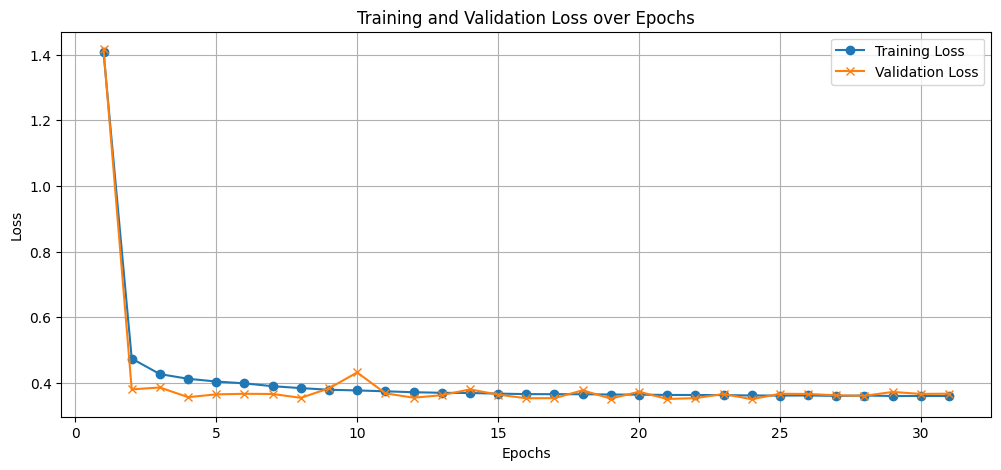
\includegraphics[width=1\linewidth]{Images/Final_Graph.png}
    \captionsetup{hypcap=false}
    \captionof{figure}{Graph of training and validation loss over epochs from the final model.}
    \label{fig:final_graph_full}
\end{center}

\begin{center}
    \begin{tabular}{| c | c |}
        \hline
        \textbf{Metric}   & \textbf{Value} \\
        \hline
        Accuracy          & 99.6901\%      \\
        \hline
        Precision (Macro) & 0.9969         \\
        Precision (Micro) & 0.9969         \\
        \hline
        Recall (Macro)    & 0.9969         \\
        Recall (Micro)    & 0.9969         \\
        \hline
        F1 Score (Macro)  & 0.9969         \\
        F1 Score (Micro)  & 0.9969         \\
        \hline
    \end{tabular}
\end{center}

\begin{center}
    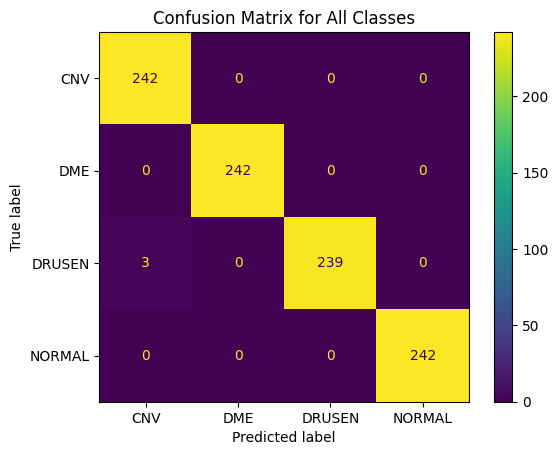
\includegraphics[width=1\linewidth]{Images/FinalMatrix.png}
    \captionsetup{hypcap=false}
    \captionof{figure}{Confusion Matrix of the test results from the final model.}
    \label{fig:final_matrix_full}
\end{center}

\subsection{Baseline and Previous Results}

\subsubsection{Baseline Results}

The baseline mode that was used for a comparison was a random classification model. This model randomly selects a class for each image without any learning or training. As a result, the expected accuracy for this model is 25\% since there are four classes.

\begin{center}
    \begin{tabular}{| c | c |}
        \hline
        \textbf{Metric}   & \textbf{Value} \\
        \hline
        Accuracy          & 25.31\%        \\
        \hline
        Precision (Macro) & 0.2527         \\
        Precision (Micro) & 0.2531         \\
        \hline
        Recall (Macro)    & 0.2531         \\
        Recall (Micro)    & 0.2531         \\
        \hline
        F1 Score (Macro)  & 0.2526         \\
        F1 Score (Micro)  & 0.2531         \\
        \hline
    \end{tabular}
\end{center}

\vfill

\begin{center}
    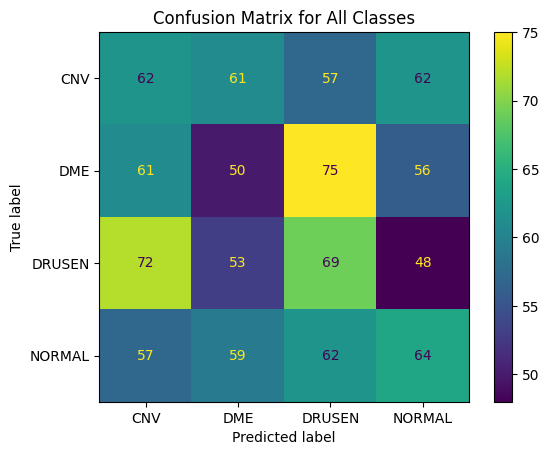
\includegraphics[width=1\linewidth]{Images/RandomMatrix.png}
    \captionsetup{hypcap=false}
    \captionof{figure}{Confusion Matrix for all classes using the random classifier.}
    \label{fig:random_matrix_full}
\end{center}

Adding onto this, each of the classes were individually evaluated. The results are shown below:

\begin{center}
    \begin{tabular}{|l|c|c|}
        \hline
        \textbf{Class}         & \textbf{Precision} & \textbf{Recall} \\
        \hline
        CNV                    & 0.25               & 0.26            \\
        DME                    & 0.22               & 0.21            \\
        DRUSEN                 & 0.26               & 0.29            \\
        NORMAL                 & 0.28               & 0.26            \\
        \hline
        \textbf{Macro Avg.}    & 0.25               & 0.25            \\
        \textbf{Weighted Avg.} & 0.25               & 0.25            \\
        \hline
    \end{tabular}
\end{center}

\begin{center}
    \begin{tabular}{|l|c|c|}
        \hline
        \textbf{Class}         & \textbf{F1-score} & \textbf{Support} \\
        \hline
        CNV                    & 0.25              & 242              \\
        DME                    & 0.22              & 242              \\
        DRUSEN                 & 0.27              & 242              \\
        NORMAL                 & 0.27              & 242              \\
        \hline
        \textbf{Accuracy}      & 0.25              & 968              \\
        \textbf{Macro Avg.}    & 0.25              & 968              \\
        \textbf{Weighted Avg.} & 0.25              & 968              \\
        \hline
    \end{tabular}
\end{center}


% Individual confusion matrices for each class
\begin{center}
    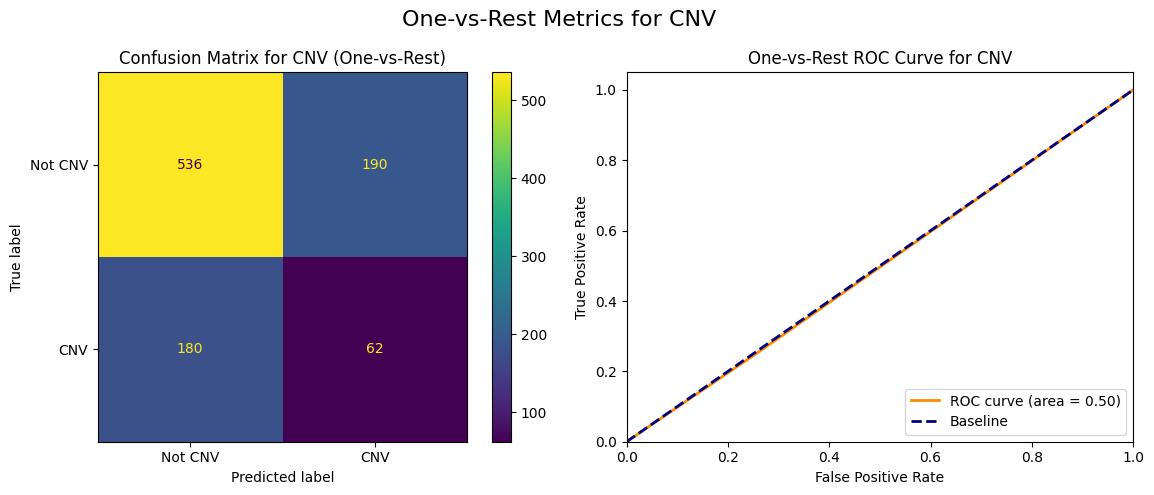
\includegraphics[width=1\linewidth]{Images/CNV_random.png}
    \captionsetup{hypcap=false}
    \captionof{figure}{Confusion Matrix for CNV class using the random classifier.}
    \label{fig:random_matrix_cnv}
\end{center}

\begin{center}
    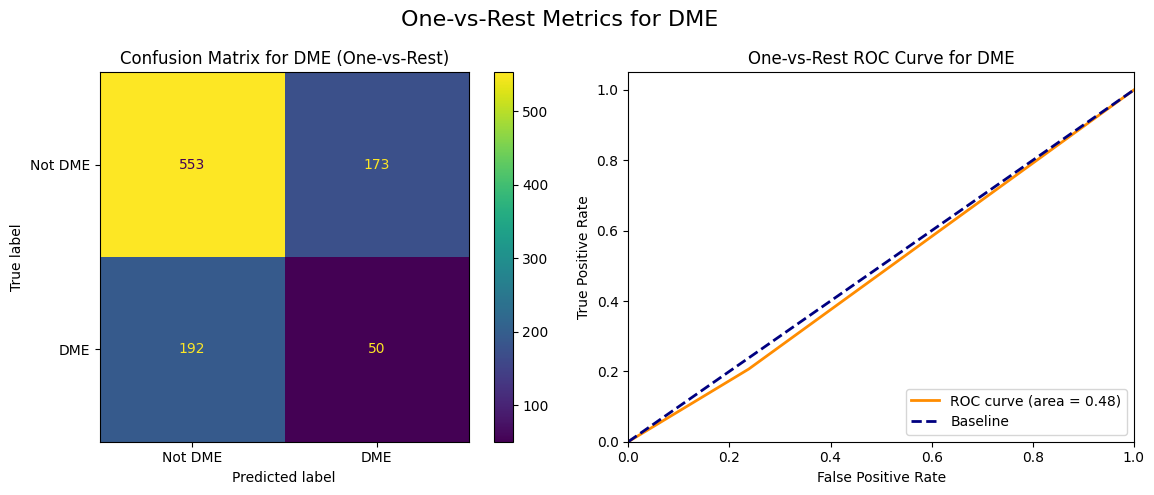
\includegraphics[width=1\linewidth]{Images/DME_random.png}
    \captionsetup{hypcap=false}
    \captionof{figure}{Confusion Matrix for DME class using the random classifier.}
    \label{fig:random_matrix_dme}
\end{center}

\begin{center}
    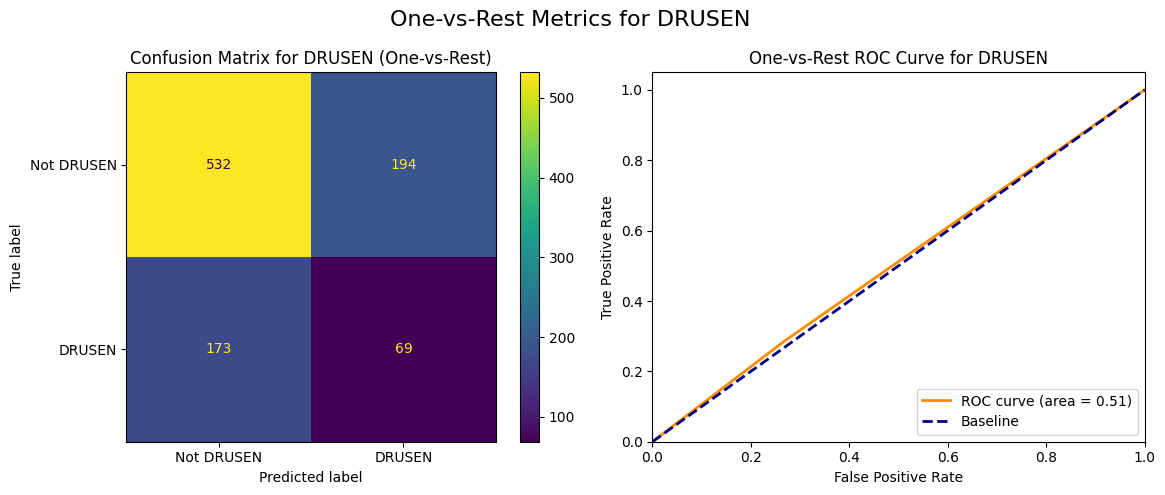
\includegraphics[width=1\linewidth]{Images/DRUSEN_random.png}
    \captionsetup{hypcap=false}
    \captionof{figure}{Confusion Matrix for DRUSEN class using the random classifier.}
    \label{fig:random_matrix_drusen}
\end{center}

\begin{center}
    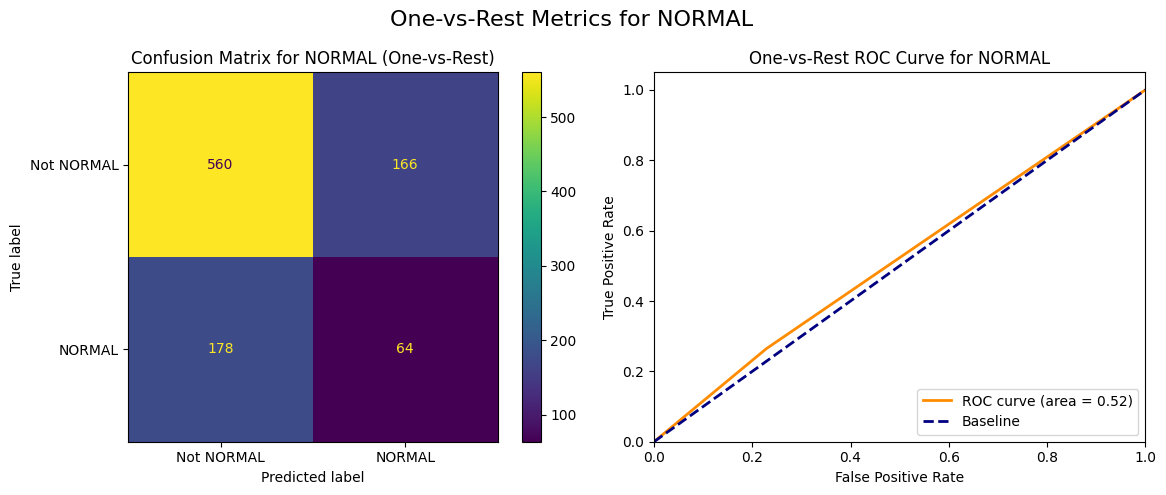
\includegraphics[width=1\linewidth]{Images/NORMAL_random.png}
    \captionsetup{hypcap=false}
    \captionof{figure}{Confusion Matrix for NORMAL class using the random classifier.}
    \label{fig:random_matrix_normal}
\end{center}


\subsubsection{Previous Results}

These are the results from the progress report. The results are not as comprehensive since many metrics such as precision and recall were not added.

\begin{center}
    \begin{tabular}{| c | c |}
        \hline
        \textbf{Metric} & \textbf{Value} \\
        \hline
        Accuracy        & 84.40\%        \\
        \hline
    \end{tabular}
\end{center}

\begin{center}
    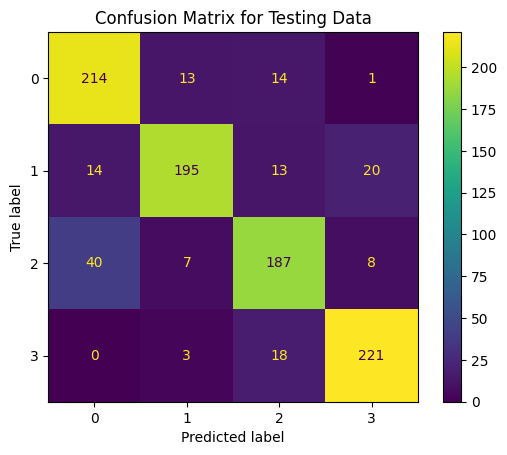
\includegraphics[width=1\linewidth]{Images/ProgressMatrix.png}
    \captionsetup{hypcap=false}
    \captionof{figure}{Confusion Matrix from the progress report.}
    \label{fig:progress_matrix_full}
\end{center}



\section{Progress}

\subsection{Feedback and Planned Improvements}

From the progress report, there were a few problems with the model and the implementation that were highlighted. To start off, the dataset for the model was imbalanced. While this was not important for the progress report since 1000 images were used for each category, this would be a problem when scaling up to a full dataset. The second issue was the lack of a baseline comparison such as Majority Class or a simple CNN. This leads into the third problem, the lack of additional metrics such as micro and macro F1 score, recall, and precision. Lastly, there was a lack of hyperparameter tuning and model optimization. There was a lack of momentum in the optimizer, and the learning rate was not adjusted throughout training.

\subsection{Implemented Improvements}

To address the issues highlighted in the feedback, the following improvements were implemented:

\subsubsection{Data Augmentation}

As highlighted in section \textbf{3.3}, data augmentation was performed to ensure a balanced dataset. Images in the other three categories (DME, DRUSEN, NORMAL) were augmented to match the number of images in CNV, which included random horizontal flips, random rotations, random resized crops, and color jittering.

\subsubsection{Additional Metrics}

The additional metrics were calculated to better evaluate the model's performance. These metrics include precision, recall, F1 score (both micro and macro), which were printed with correspondence with the confusion matrix. These metrics provide a more comprehensive understanding of the model's strengths and weaknesses across different classes.

\subsubsection{Baseline Comparison}

To address the lack of a baseline comparison, a random classifier was used as a baseline. This classifier

\subsubsection{Hyperparameter Tuning}

To help the model achieve better performance, several model optimizations and hyperparameter tuning were conducted. Including ones that involved planning, like the addition of momentum in the optimizer and learning rate adjustments and tuning in the form of the learning rate scheduler, and ones that were not planned, like the transition from the Adam optimizer to SGD, the early-stopping, and the unfreezing of the last three layers of the ResNet-50 model, in addition to the classifier. The reason for the extra additions is that research during the fine-tuning and optimization process revealed improvements that not only improved the model's generalization, leading to better performance, but also accelerated convergence, which was a priority given the dataset's massive size, resulting in long computation time. Furthermore, as the Applications of Machine Learning course progressed, more information regarding ways to improve a model was discovered that helped influence the optimizations and additions made to the model. For a full breakdown of the hyperparameter tuning and model optimizations implemented, as well as the reasoning behind the choices, please refer to section 5.2.

\subsection{Progress Evaluation}

When viewing all the feedback and the implemented improvements, all the proposed feedback and plans were implemented. There was no change in course of action because the final test accuracy for the model was 99.69\%, thus hitting the initial target proposed.


\section{Error Analysis}


\begin{figure}[h!]
    \centering
    \scriptsize % Make all text and tables smaller
    \begin{multicols*}{2}
        \centering
        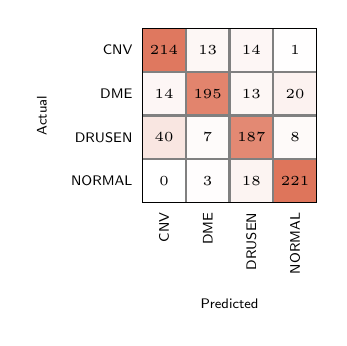
\begin{tikzpicture}
            \begin{axis}[
                    width=3.8cm, height=3.8cm,
                    colormap={Red}{color=(white) rgb255=(222, 117, 91)},
                    xlabel=Predicted,
                    xlabel style={yshift=-2pt, font=\tiny},
                    ylabel=Actual,
                    ylabel style={yshift=2pt, font=\tiny},
                    xticklabels={CNV, DME, DRUSEN, NORMAL},
                    xtick={0,...,3},
                    xtick style={draw=none},
                    yticklabels={CNV, DME, DRUSEN, NORMAL},
                    ytick={0,...,3},
                    ytick style={draw=none},
                    enlargelimits=false,
                    colorbar=false,
                    tick label style={font=\tiny},
                    xticklabel style={rotate=90, font=\tiny},
                    yticklabel style={font=\tiny},
                    nodes near coords={\pgfmathprintnumber\pgfplotspointmeta},
                    every node near coord/.append style={anchor=center, font=\tiny},
                ]
                \addplot[
                    matrix plot,
                    mesh/cols=4,
                    point meta=explicit,
                    draw=gray,
                    thick=0.3pt,
                ] table [meta=C] {
                        x y C
                        0 0 214
                        1 0 13
                        2 0 14
                        3 0 1

                        0 1 14
                        1 1 195
                        2 1 13
                        3 1 20

                        0 2 40
                        1 2 7
                        2 2 187
                        3 2 8

                        0 3 0
                        1 3 3
                        2 3 18
                        3 3 221
                    };
            \end{axis}
        \end{tikzpicture}

        a. Progress Report Model

        \centering

        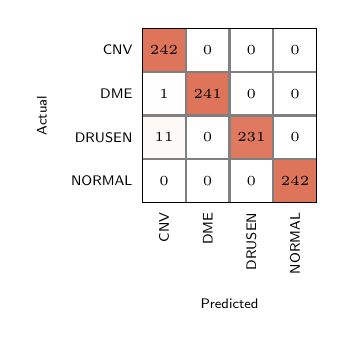
\begin{tikzpicture}
            \begin{axis}[
                    width=3.8cm, height=3.8cm,
                    colormap={Red}{color=(white) rgb255=(222, 117, 91)},
                    xlabel=Predicted,
                    xlabel style={yshift=-2pt, font=\tiny},
                    ylabel=Actual,
                    ylabel style={yshift=2pt, font=\tiny},
                    xticklabels={CNV, DME, DRUSEN, NORMAL},
                    xtick={0,...,3},
                    xtick style={draw=none},
                    yticklabels={CNV, DME, DRUSEN, NORMAL},
                    ytick={0,...,3},
                    ytick style={draw=none},
                    enlargelimits=false,
                    colorbar=false,
                    tick label style={font=\tiny},
                    xticklabel style={rotate=90, font=\tiny},
                    yticklabel style={font=\tiny},
                    nodes near coords={\pgfmathprintnumber\pgfplotspointmeta},
                    every node near coord/.append style={anchor=center, font=\tiny},
                ]
                \addplot[
                    matrix plot,
                    mesh/cols=4,
                    point meta=explicit,
                    draw=gray,
                    thick=0.3pt,
                ] table [meta=C] {
                        x y C
                        0 0 242
                        1 0 0
                        2 0 0
                        3 0 0

                        0 1 1
                        1 1 241
                        2 1 0
                        3 1 0

                        0 2 11
                        1 2 0
                        2 2 231
                        3 2 0

                        0 3 0
                        1 3 0
                        2 3 0
                        3 3 242
                    };
            \end{axis}
        \end{tikzpicture}

        b. Final Report Model (1000 per Category)

        \centering

    \end{multicols*}

    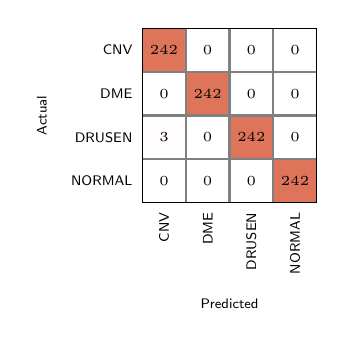
\begin{tikzpicture}
        \begin{axis}[
                width=3.8cm, height=3.8cm,
                colormap={Red}{color=(white) rgb255=(222, 117, 91)},
                xlabel=Predicted,
                xlabel style={yshift=-2pt, font=\tiny},
                ylabel=Actual,
                ylabel style={yshift=2pt, font=\tiny},
                xticklabels={CNV, DME, DRUSEN, NORMAL},
                xtick={0,...,3},
                xtick style={draw=none},
                yticklabels={CNV, DME, DRUSEN, NORMAL},
                ytick={0,...,3},
                ytick style={draw=none},
                enlargelimits=false,
                colorbar=false,
                tick label style={font=\tiny},
                xticklabel style={rotate=90, font=\tiny},
                yticklabel style={font=\tiny},
                nodes near coords={\pgfmathprintnumber\pgfplotspointmeta},
                every node near coord/.append style={anchor=center, font=\tiny},
            ]
            \addplot[
                matrix plot,
                mesh/cols=4,
                point meta=explicit,
                draw=gray,
                thick=0.3pt,
            ] table [meta=C] {
                    x y C
                    0 0 242
                    1 0 0
                    2 0 0
                    3 0 0

                    0 1 0
                    1 1 242
                    2 1 0
                    3 1 0

                    0 2 3
                    1 2 0
                    2 2 242
                    3 2 0

                    0 3 0
                    1 3 0
                    2 3 0
                    3 3 242
                };
        \end{axis}
    \end{tikzpicture}

    c. Final Report Model (All Images)
    \caption{Confusion matrices for three models generated by group 76: Progress Report Model, Final Report Model (1000 per Category), and the Final Report Model (All Images).}
    \label{fig:comparison_model_matrices}
\end{figure}

\begin{figure}[h!]
    \centering
    \begin{minipage}[b]{0.49\linewidth}
        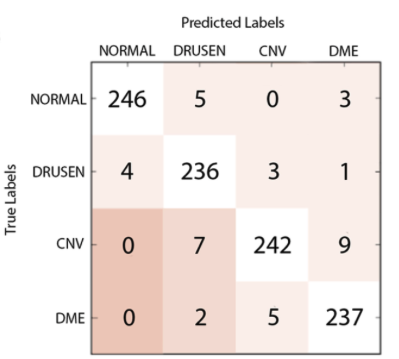
\includegraphics[width=\linewidth]{Images/KermanyMatrix.png}
        \captionsetup{hypcap=false}
    \end{minipage}
    \hfill
    \begin{minipage}[b]{0.49\linewidth}
        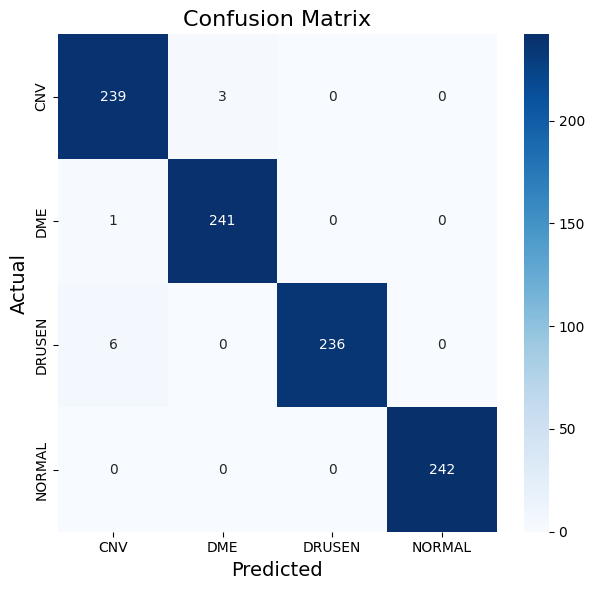
\includegraphics[width=\linewidth]{Images/ReddyMatrix.png}
        \captionsetup{hypcap=false}
    \end{minipage}
    \caption{Confusion matrices from models outlined in~\citep{Kermany2018-dc} and~\citep{Reddy_2025-nr}.}
    \label{fig:comparison_reddy_kermany_matrices}
\end{figure}

\begin{center}
    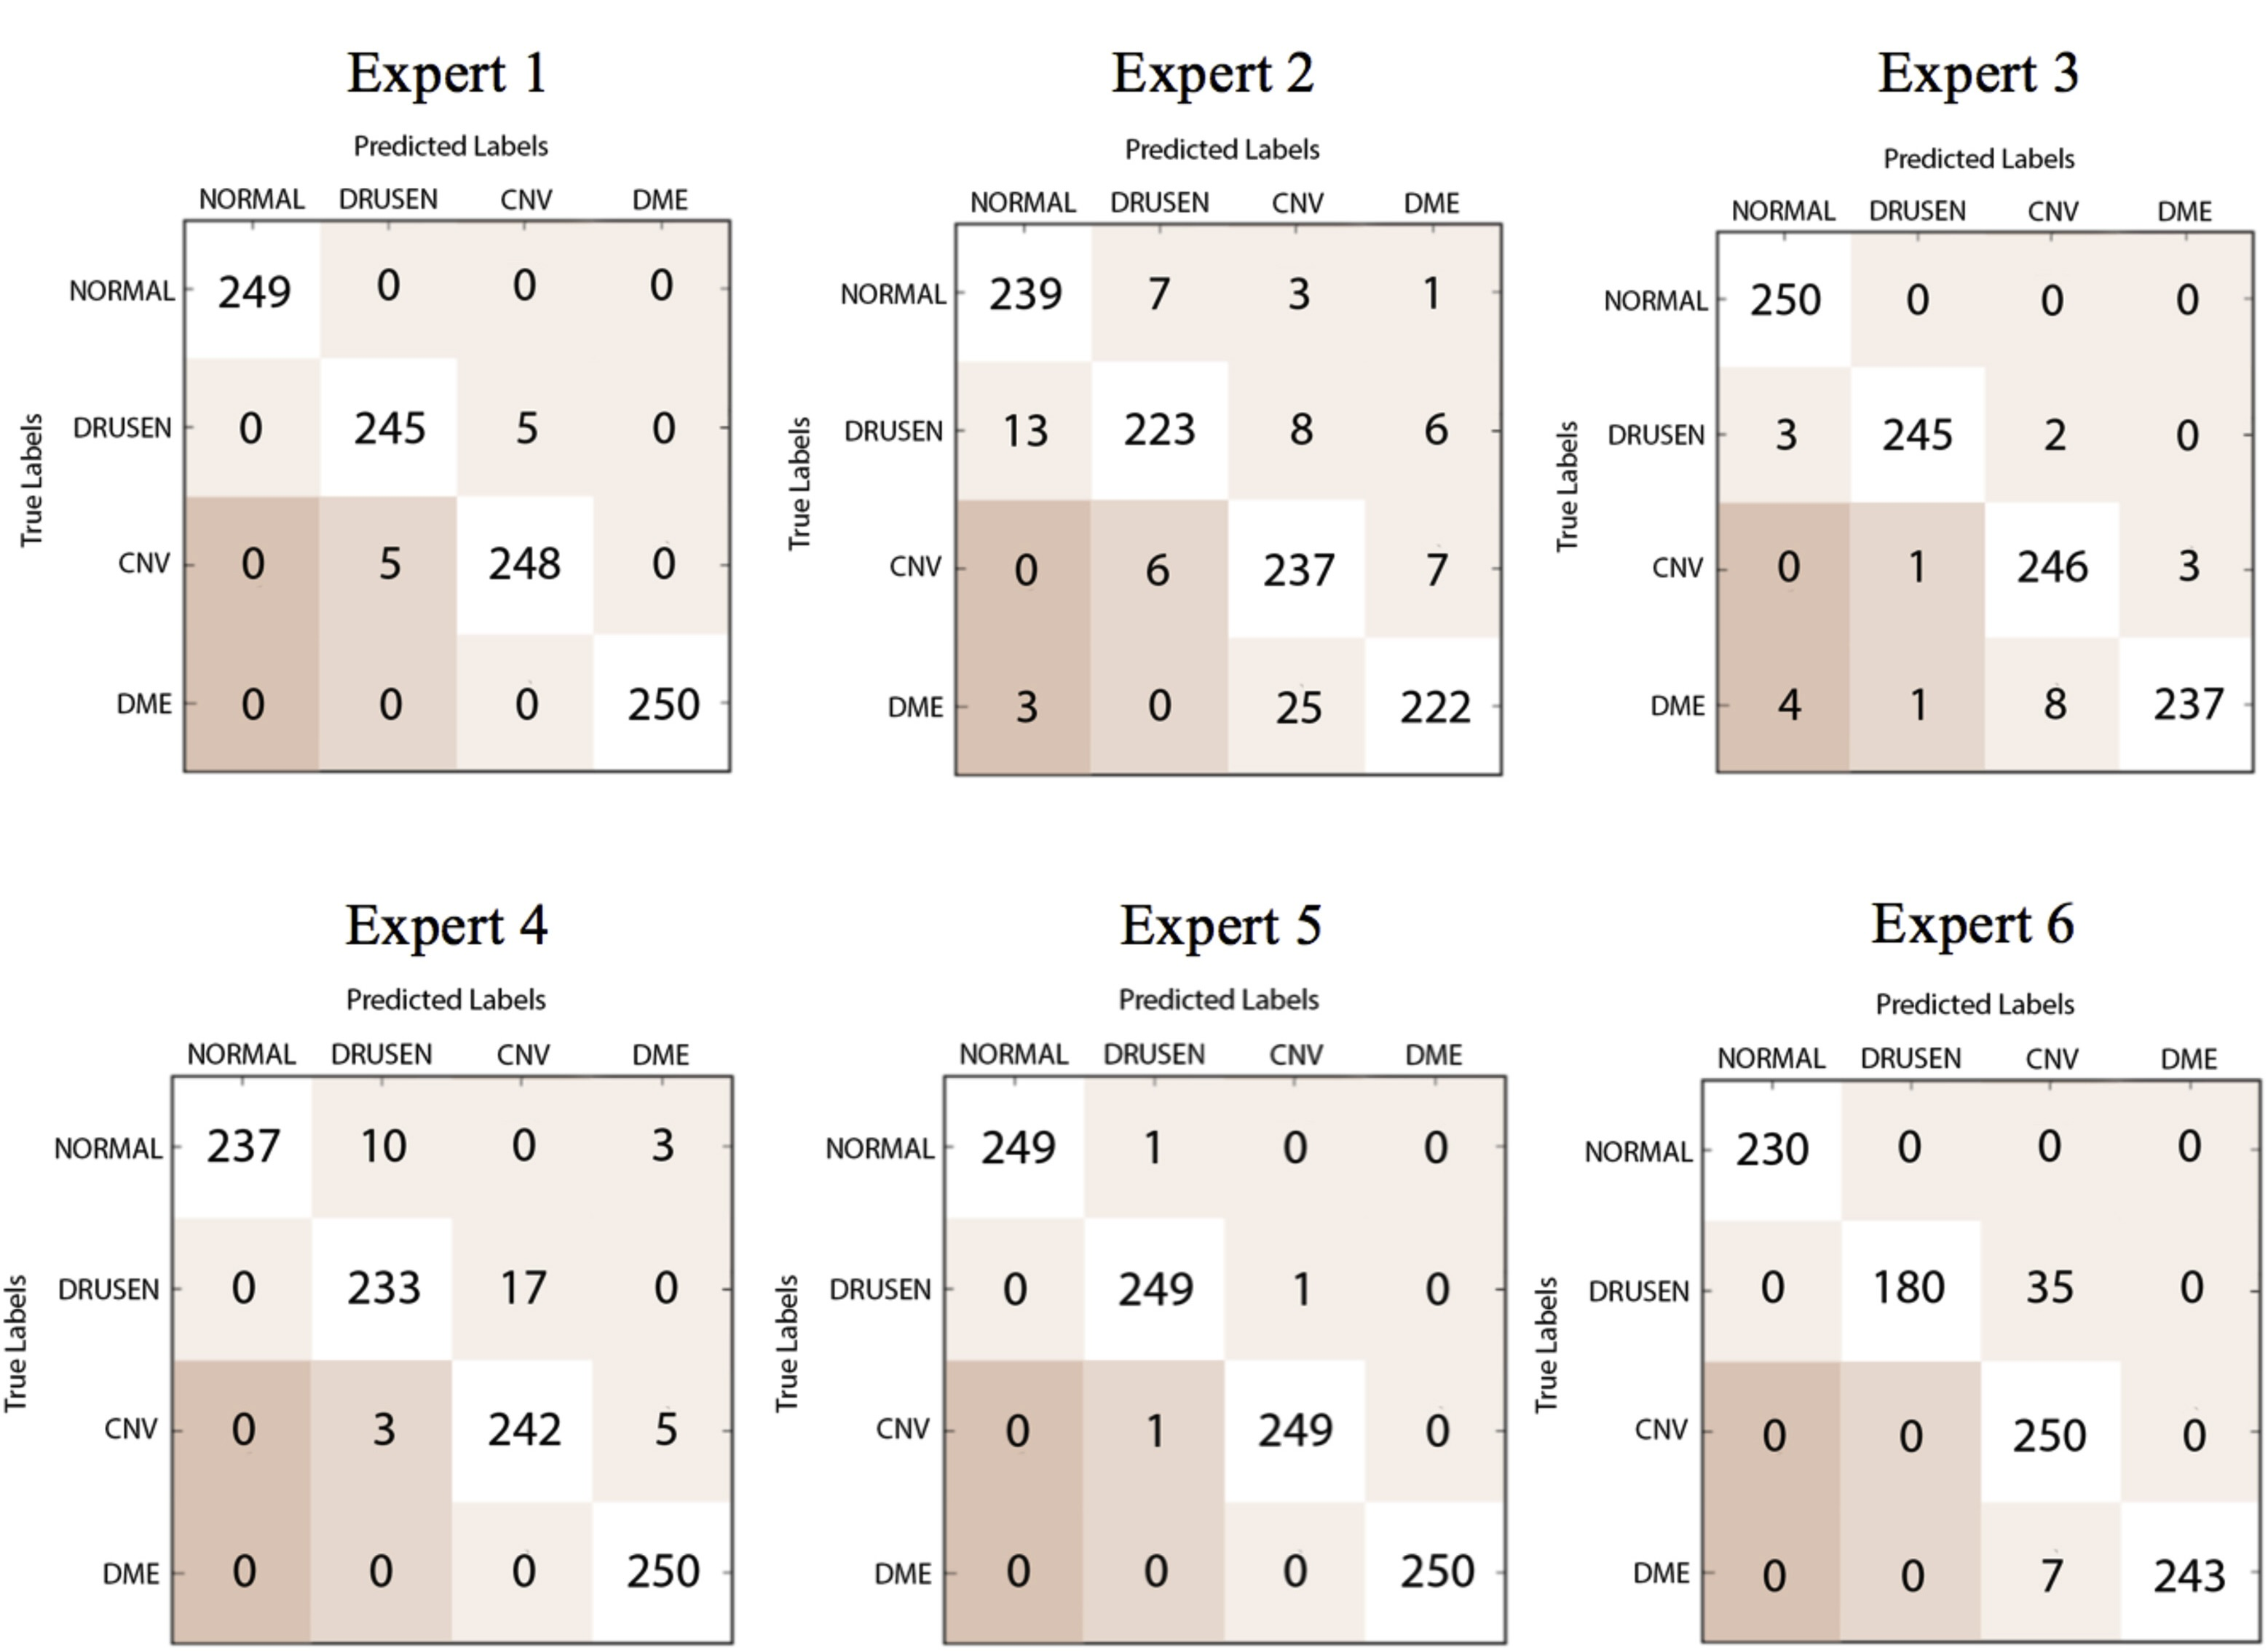
\includegraphics[width=1\linewidth]{Images/6Matrix.png}
    \captionsetup{hypcap=false}
    \captionof{figure}{Confusion Matrix from the progress report.}
    \label{fig:kermany_human_full}
\end{center}


As shown in section 6.3 and figure 9, the final model was able to perform incredibly well, only making 3 wrong predictions out of all 968 data points in the test set. It was also able to reach a perfect 1.0 recall, precision, and f-1 scores for the NORMAL-vs-Rest classification. This means that all cases of a retinal disease would be classified as a disease, which will help the early detection of retinal diseases and hopefully prevent any condition from being undiagnosed. Comparing this to the results shown in Kermany et al.~\citeyearpar{Kermany2018-dc} and Reddy~\citeyearpar{Reddy_2025-nr}, it can be seen that the model seems to outperform most if not all of these implementations, including human experts.

On the other hand, figure 9 clearly shows that the final results for the model trained on all the images has only 3 incorrect predictions, all of which come from DRUSEN images that were classified as CNV. This is a pattern that can be seen throughout the different versions of the model's implementation and in the results from Kermany et al.~\citeyearpar{Kermany2018-dc} and Reddy~\citeyearpar{Reddy_2025-nr} as seen in figures 10. This bias towards predicting CNV could be caused by the distribution of the training dataset itself which has a lot more CNV images. While data augmentation was performed to get DME and DRUSEN's data to be the same amount as CNV, these newly added data were essentially slight modifications to the original and much smaller dataset. Thus, it is possible that the model had a harder time learning the features of DME and DRUSEN when compared to CNV. However, it can be seen in figure 11 that human experts also tend to mostly misclassify a DME and DRUSEN as CNV, which could suggest that the bias that is seen in the model is a result of the characteristics of the underlying problem itself.

One thing that can be done to possibly improve the model and mitigate this bias is to downsample the majority class, which in this case is the CNV class. By downsampling it, there will be less data augmentation required for the other classes such as DME and DRUSEN. An experiment can be conducted to see if different distributions of augmented vs non-augmented data change the bias of the predictions that the model makes. However, it must be noted that while downsampling the dataset might fix the bias issue, it is also important to keep a large enough dataset for each class so that the model can still learn the required features to perform its task.

\section{Team Contributions}

\subsection{Elite}

\begin{itemize}
    \item Worked on the initial image opening and storing of data.
    \item Implemented the image augmentation process.
    \item Wrote sections 1, 3, 4, 5, and 7 of the document and worked on overall presentation of Latex
\end{itemize}

\subsection{Ishpreet}

\begin{itemize}
    \item Implemented the ResNet-50 neural network and its corresponding training, validation, and testing codes.
    \item Performed hyperparameter tuning and model optimizations.
    \item Trained, validated, and tested the model.
    \item Wrote sections 5.2.3, 5.2.4, 5.2.5, and 7.2.4 of the document.
\end{itemize}

\subsection{Kenneth}

\begin{itemize}
    \item Worked on setting up the neural network and research for the start of the project.
    \item Implemented the initial data preprocessing pipeline.
    \item Implemented the evaluation metrics and confusion matrix plotting.
    \item Wrote sections 2, 6, and 8 of the document.
\end{itemize}

\bibliography{custom}

\end{document}
